\documentclass[a4paper,12pt]{article}
\usepackage{graphicx}
\usepackage{hyperref}   % use for hypertext links, including those to external documents and URLs

\begin{document}



\begin{center}
\begin{Huge}
\textbf{{\LARGE Unit Test Visuliation\\Installation Guide }}
\linebreak
\linebreak
\linebreak
\linebreak
\end{Huge}\end{center}




\begin{small}
\begin{flushleft}
\textbf{Author:} Keagan Phillips
\\
\textbf{Team:} Group 4
\\
\textbf{Course:} ELEN7046 - Software Technologies and Techniques
\\
\textbf{Date Submitted:} 25 June 2012
\\
\textbf{Source \& Documentation:} https://github.com/KeaganPhillips/Wit-Group-4-project/tree/master/Documentation
\linebreak
\linebreak
\linebreak
\linebreak
\linebreak
\end{flushleft}

\end{small}


\begin{flushleft}
\textbf{{\large Abstract}}
\end{flushleft}
This document outlines the processes and procedures required to deploy and configure of the "Unit Test Visualistion" system to the desired environment. It covers the assumptions made about the target platform, system requirements and the installation procedure among other topics related to the installation of the above system.
\clearpage


\tableofcontents
\clearpage


\section{Introduction}
\subsection{Overview}
This document serves as an installation guide for the "Unit Test Visualistion" system. The application is web based and was developed using Microsoft Visual Studio 2010\cite{vs2010} using the C\# programming language. 

\section{Platform}
The system was developed using the Dot Net Framework 4.0\cite{dotNet} and is intended to run on a Microsoft Windows\cite{windows} based operating system. (i.e. Windows XP / Windows Server 2003 / Windows 7). 


\section{System Requirements}
\subsection{Hardware Requirements}
The application to be installed is not very systems resource intensive and should work well on any modern (not older than 7 years from) server/PC. An Intel Pentium Celeron processor with 2 GB RAM and 100 MB free space should be sufficient. 
\subsection{Software Requirements}
The authors do assume that the target system has the following components installed and fully configured.
\begin{itemize}

\item Microsoft Dot Net Framework 4.0 \cite{dotNet}
\item Microsoft IIS 7 \cite{iis}

\end{itemize}


\section{Installation Procedure}
The following lists the steps needed to install the system on the targeted server.
\begin{enumerate}
\item Create a new folder on the target server where the application will be copied to. (e.g. "C:\textbackslash intepub\textbackslash wwwroot\textbackslash UnitTestVisualiser")
\item From within Visual Studio 2010\cite{vs2010}, publish your Web application by right clicking on the web application project and clicking the publish context menu item.
\item XCopy the content of the published project to the target folder.
\item From the start run console enter inetmgr and hit Enter. IIS manager should appear as shown in Figure \ref{fig1}. Browse to the UnitTestVisualiser folder right click on it and select 'Convert to Application' as shown in Figure \ref{fig2}
\item Ensure that the application uses a Dot Net Framework 4.0 application pool by using an existing application pool or by creating a new application pool.
\item Make sure the web application is up an running by pointing your browser to the site and by clicking through the application. The URL should resemble something like (http://servername:80/UnitTestVisualiser). The servername and port number depends on your specific environment and configuration.
\end{enumerate}

\section{Conclusion}
That concludes the installation procedure required for the installation of the Unit test visualisation application on your targeted server.

\begin{center}
	\begin{figure}
		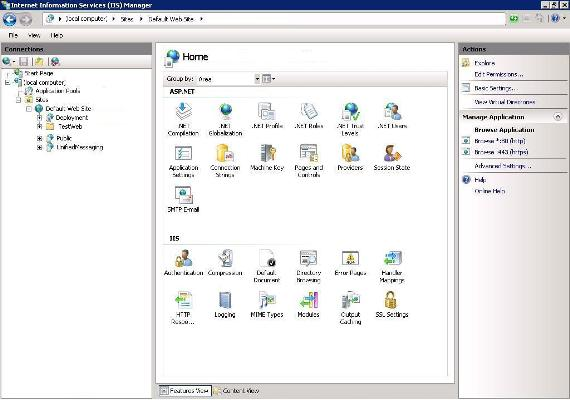
\includegraphics{Main_DefaultIIS.JPG}
			\caption{}
			\label{fig1}    
	\end{figure}	
\end{center}

\begin{center}
	\begin{figure}
		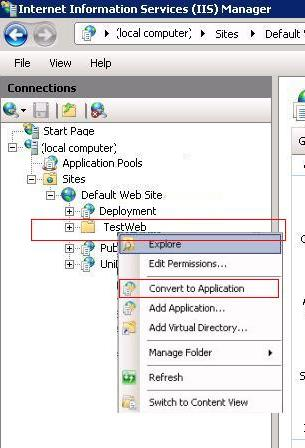
\includegraphics{ConvertToApplication.JPG}
			\caption{}
			\label{fig2}    
	\end{figure}	
\end{center}

\clearpage
\begin{thebibliography}{5}

\bibitem{vs2010} \begin{flushleft}
Microsoft Visual Studio; Wikipedia
\end{flushleft} \url{http://en.wikipedia.org/wiki/Microsoft_Visual_Studio}

\bibitem{dotNet}\begin{flushleft}
 The .NET Framework 4; MSDN 
\end{flushleft}\url{http://msdn.microsoft.com/en-us/library/w0x726c2.aspx}

\bibitem{windows}\begin{flushleft}
 Microsoft Windows Operating systems; wikipedia
\end{flushleft} \url{http://en.wikipedia.org/wiki/Microsoft_Windows}

\bibitem{iis} \begin{flushleft}
Web Server (IIS); technet.microsoft.com 
\end{flushleft}\url{http://technet.microsoft.com/en-us/library/cc753433%28v=ws.10%29}

\end{thebibliography}


 


\end{document}